\documentclass[conference]{IEEEtran}
\IEEEoverridecommandlockouts

% =========================================================
% PACKAGES
% =========================================================
\usepackage{cite}
\usepackage{amsmath,amssymb,amsfonts}
\usepackage{algorithmic}
\usepackage{graphicx}
\usepackage{textcomp}
\usepackage{xcolor}
\usepackage{listings}
\usepackage{hyperref}
\usepackage{booktabs}
\usepackage{multirow}
\usepackage{array}
\usepackage{float}
\usepackage{placeins} % provides \FloatBarrier to prevent floats entering references
\usepackage{placeins}  % For \FloatBarrier command

% TikZ and Plotting Settings
\usepackage{tikz}
\usetikzlibrary{
  shapes.geometric,
  shapes.arrows,
  shapes.multipart,
  arrows.meta,
  positioning,
  fit,
  backgrounds,
  calc,
  shadows,
  shadows.blur,
  patterns,
  decorations.pathreplacing,
  decorations.pathmorphing,
  decorations.markings
}
\usepackage{pgfplots}
\pgfplotsset{compat=1.18}

% Professional Color Palette
\definecolor{primary}{RGB}{0, 85, 128}      % Deep Blue
\definecolor{secondary}{RGB}{0, 139, 139}   % Teal
\definecolor{accent}{RGB}{205, 92, 92}      % Indian Red
\definecolor{highlight}{RGB}{255, 165, 0}   % Orange
\definecolor{lightgray}{RGB}{245, 245, 245}
\definecolor{p1color}{RGB}{100, 149, 237}   % CornflowerBlue
\definecolor{p2color}{RGB}{255, 160, 122}   % LightSalmon
\definecolor{abccolor}{RGB}{147, 112, 219}  % Medium Purple for ABC

% =========================================================
% MACROS
% =========================================================
\newcommand{\systemname}{MAESTRO}
% =========================================================
% DOCUMENT START
% =========================================================
\begin{document}

\title{Meta-heuristic Adaptive Exploration Strategy Through Routing Optimization}


\author{\IEEEauthorblockN{Ahd Mostafa\IEEEauthorrefmark{1}, Amr Hegazy\IEEEauthorrefmark{1}, Fathy Ashraf\IEEEauthorrefmark{1}, Mohamed Wael\IEEEauthorrefmark{1}, Youssef Elbrolosy\IEEEauthorrefmark{1}, Ziad Abdelrahman\IEEEauthorrefmark{1}}
\IEEEauthorblockA{\textit{Faculty of Media Enginerring \& Technology (CSEN), Faculty of Engineering and Materials Science (MCTR)} \\
\textit{The German University in Cairo}\\
Cairo, Egypt \\
\{ahd.mostafa, amr.hazem, fathy.ashraf, mohamed.wael, youssef.elbrolosy, ziad.abdelrahman\}@student.guc.edu.eg}
\IEEEauthorblockA{\IEEEauthorrefmark{1}These authors contributed equally to this work.}
}

\maketitle

\begin{abstract}
Efficient exploration of unknown environments by multi-robot teams requires a delicate balance between coverage maximization and the maintenance of communication connectivity. While various metaheuristic approaches such as Genetic Algorithms (GA), Ant Colony Optimization (ACO), Simulated Annealing (SA), and Artificial Bee Colony (ABC) have been applied to this problem, no single algorithm dominates across all environmental conditions. In sparse environments, constructive methods like ACO often excel, whereas perturbative methods like SA may offer superior computational efficiency in simpler scenarios. We introduce \textbf{\systemname{}}, a framework that integrates a learned router (Random Forest) to dynamically select the optimal planner based on extracted map features and connectivity/topology statistics. Our evaluation, performed on a dataset of 1,836 test scenarios, demonstrates that this adaptive approach achieves a classification accuracy of \textbf{94.99\%} in selecting the optimal solver. We further conduct a sensitivity analysis on GA population sizing, proving that adaptive routing outperforms even hyperparameter-tuned static solvers. Crucially, the system exhibits a "fail-safe" property: in our testing, it \textbf{never} incorrectly selected the lightweight solver (SA) for complex instances requiring robust optimization (ACO), thereby minimizing mission failure risk while reducing computational overhead by approximately 34\%.
\end{abstract}

\begin{IEEEkeywords}
Multi-Robot Systems, Path Planning, Metaheuristics, Adaptive Selection, Connectivity Maintenance, Learning to Optimize.
\end{IEEEkeywords}

\section{Introduction}
\label{sec:introduction}

The deployment of Multi-Robot Systems (MRS) for search and rescue operations relies on the team's ability to maximize area coverage while adhering to strict operational constraints. Foremost among these is the requirement for network connectivity \cite{li2008swarm}, which ensures that critical data discovered by any agent can be transmitted to a base station or shared among peers. However, the objectives of coverage and connectivity are inherently conflicting: maximizing coverage drives robots apart to explore new frontiers, while connectivity constraints pull them together to maintain communication links \cite{yamauchi1997frontier}.

This optimization problem is NP-hard, prompting the widespread adoption of metaheuristic solvers. Evolutionary approaches, such as Genetic Algorithms (GA), offer robust exploration of the solution space but suffer from high computational costs due to population management \cite{deb2023multi}. Conversely, constructive methods like Ant Colony Optimization (ACO) excel at identifying high-quality paths through pheromone feedback loops but can be computationally prohibitive for real-time applications \cite{dorigo2024aco}. Trajectory-based methods like Simulated Annealing (SA) provide a lightweight alternative but are prone to entrapment in local optima \cite{kirkpatrick2021sa}.

Recent literature typically proposes a single "best" algorithm for a specific domain. However, real-world deployment scenarios vary drastically, from open fields with few obstacles to dense urban rubble. A "one-size-fits-all" algorithm inevitably leads to either computational waste (using a heavy solver for a simple problem) or solution degradation (using a weak solver for a hard problem). This limitation has spurred interest in "Learning to Optimize" (L2O) strategies, where the optimizer itself is selected or tuned based on problem features \cite{chen2022learning}.

We introduce \textit{\systemname{}}, an adaptive path planning framework that utilizes a machine learning router to select the most appropriate metaheuristic for a given scenario. By characterizing the problem instance through topological features, our system intelligently switches between SA, GA, ACO, and ABC.

Our specific contributions are:
\begin{enumerate}
    \item \textbf{Unified Framework}: A formulation of the connectivity-aware exploration problem supporting interchangeable optimization backends (SA, GA, ACO, ABC).
    \item \textbf{Learned Routing}: A feature-based Random Forest router that predicts solver performance with 94.99\% accuracy based on metrics such as obstacle fraction and connectivity graph density.
    \item \textbf{Fail-Safe Validation}: An extensive analysis of failure modes, demonstrating zero critical routing errors (assigning weak solvers to hard problems) on a large test set.
    \item \textbf{Hyperparameter Sensitivity Study}: A comparative analysis demonstrating that routing provides better performance gains than simply tuning static solver parameters (e.g., GA population size).
\end{enumerate}

\section{Related Work}
\label{sec:related}

\subsection{Connectivity-Aware Exploration}
The foundational paradigm for autonomous exploration is frontier-based allocation, established by Yamauchi \cite{yamauchi1997frontier}. While effective, early methods often treated connectivity as a secondary soft constraint. More recent approaches explicitly incorporate connectivity maintenance into exploration and task allocation strategies \cite{yan2023cooperative}. Our work adopts a distance-weighted link-quality model that is inexpensive to evaluate within iterative metaheuristics.

\subsection{Metaheuristics in Path Planning}
Bio-inspired algorithms are standard for MRS path planning. GA has shown success in evolving trajectories, though maintaining kinematic feasibility during crossover remains a challenge \cite{huang2020coverage}. ACO is widely adopted for grid-based planning due to its natural graph representation \cite{dorigo2024aco}. Recent hybrid approaches, such as the Advanced Multi-Objective Salp Swarm Algorithm \cite{amet2025}, demonstrate that combining deterministic coordination with stochastic optimization improves scalability. However, comparative studies like those by Kashyap et al. \cite{kashyap2025simulations} often seek a single winner based on average performance, ignoring that algorithm ranking often flips based on environmental topology.

\subsection{Algorithm Selection and Learning to Optimize}
The "Algorithm Selection Problem," first formalized by Rice \cite{rice1976algorithm}, has seen renewed interest with the rise of "Learning to Optimize" (L2O) \cite{chen2022learning}. Hutter et al. \cite{hutter2014algorithm} demonstrated that empirical performance models can accurately predict runtime and solution quality based on instance features. In the database domain, Zhu et al. \cite{zhu2023lero} proposed pairwise ranking for query optimizer selection. Our approach applies supervised classification to select the best solver from a portfolio *a priori*, minimizing the initialization overhead associated with hyper-heuristics that switch strategies online.

\section{System Methodology}
\label{sec:methodology}

\subsection{Problem Formulation}
We consider a team of $R$ identical robots exploring an (initially unknown) discrete grid map
$M \in \{0,1\}^{H\times W}$ (0: free, 1: obstacle). The position of robot $i$ at time $t$ is
$p_{i,t}=(x_{i,t},y_{i,t})\in\{1,\ldots,H\}\times\{1,\ldots,W\}$, with given initial positions
$\{p_{i,0}\}_{i=1}^R$. Robots move synchronously on a 4-connected grid:
\begin{equation}
    \lVert p_{i,t}-p_{i,t-1}\rVert_1 \le 1,\quad \forall i\in\{1,\ldots,R\},\; \forall t\ge 1 .
\end{equation}
Each robot has an energy budget $E$ (maximum number of cell moves),
\begin{equation}
    D_{i,T}=\sum_{t=1}^{T}\lVert p_{i,t}-p_{i,t-1}\rVert_1 \le E,\quad \forall i .
\end{equation}
Let $C(P)=\bigcup_{i=1}^{R}\bigcup_{t=0}^{T}\{p_{i,t}\}$ be the set of covered cells.

Connectivity is modeled via a distance-weighted link quality between robot pair $(i,j)$:
\begin{equation}
    w_{ij}(t)=
    \begin{cases}
    \dfrac{1}{1+d_{ij}(t)}, & d_{ij}(t)\le r,\\
    0, & \text{otherwise,}
    \end{cases}
\end{equation}
where $d_{ij}(t)=\lVert p_{i,t}-p_{j,t}\rVert_2$ and $r$ is the communication radius. We also form a
communication graph $G_t$ with an edge $(i,j)$ if $d_{ij}(t)\le\tau$ (connectivity threshold). Robots
outside the largest connected component incur a disconnection penalty proportional to their distance to
the main network:
\begin{equation}
    P_{\text{disconnect}}=\sum_{t=0}^{T}\sum_{i=1}^{R}\delta_{i,t}\,d_{i,\text{net}}(t),
\end{equation}
where $\delta_{i,t}\in\{0,1\}$ indicates disconnection at time $t$, and $d_{i,\text{net}}(t)$ is the
minimum distance from robot $i$ to any robot in the main component.

We minimize a composite objective (lower is better):
\begin{equation}
    J(P)=
    \frac{\alpha}{|C(P)|+\epsilon}
    +\frac{\beta}{\sum_{t}\sum_{i<j} w_{ij}(t)+\epsilon}
    +\gamma\cdot P_{\text{disconnect}},
\end{equation}
subject to standard feasibility constraints (map bounds, obstacle avoidance, and no same-cell collisions).
The weights $\alpha,\beta,\gamma$ trade off coverage, connectivity, and robustness to network fragmentation,
and $\epsilon$ is a small constant for numerical stability.

\subsection{System Architecture}
The \systemname{} architecture (Fig.~\ref{fig:architecture}) operates in three stages. First, the \textbf{Feature Extractor} analyzes the map and initial robot configuration. Second, the \textbf{Router} (a pre-trained classifier) predicts which optimizer is best suited for the instance. Finally, the selected \textbf{Optimizer} executes the search.
\FloatBarrier

\begin{figure*}
\centering
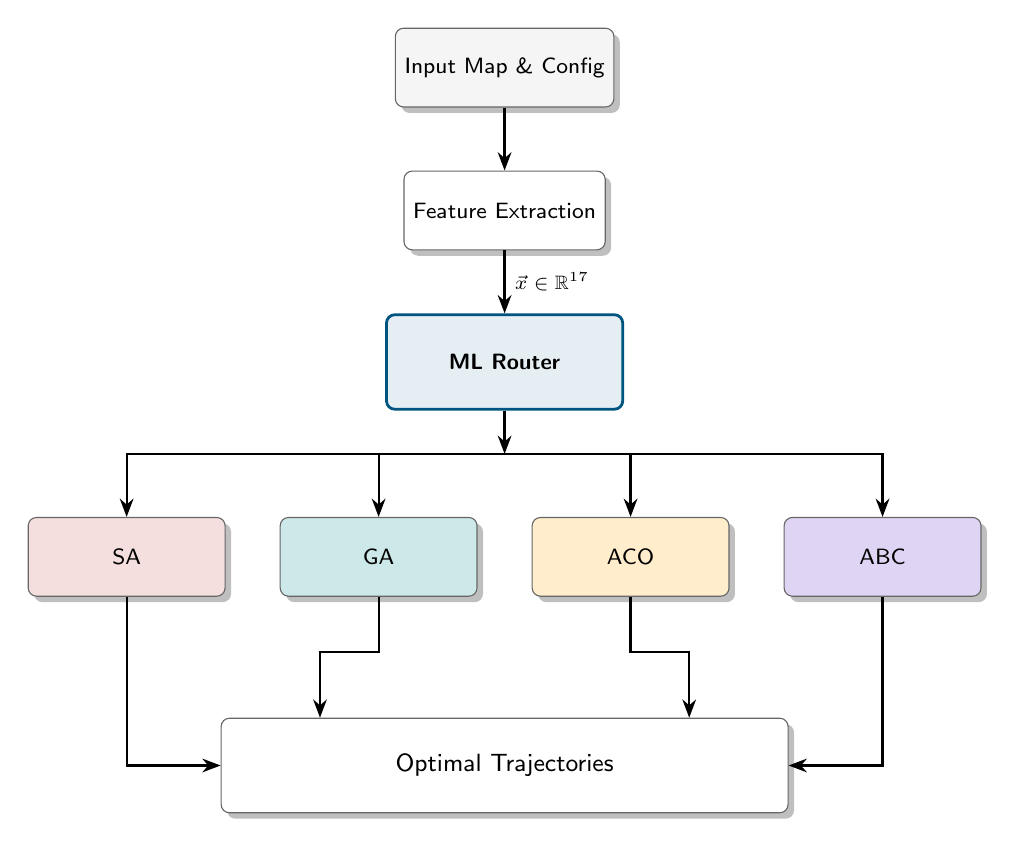
\begin{tikzpicture}[
  node distance=0.8cm,
  every node/.style={font=\sffamily\footnotesize}
]
  % Styles
  \tikzstyle{block} = [rectangle, rounded corners=3pt, minimum width=2.5cm, minimum height=1.0cm, text centered, draw=black!60, fill=white, drop shadow]
  \tikzstyle{router} = [rectangle, rounded corners=3pt, minimum width=3cm, minimum height=1.2cm, text centered, draw=primary, fill=primary!10, line width=1pt]
   
  % Input
  \node[block, fill=lightgray] (input) {Input Map \& Config};
  \node[block, below=of input] (features) {Feature Extraction};
  \node[router, below=of features] (router) {\shortstack{\textbf{ML Router}}};
   
  % Optimizers (Parallel) - centered row under the router
  \node[block, below=1.35cm of router, xshift=-4.8cm, fill=accent!20] (sa) {SA};
  \node[block, below=1.35cm of router, xshift=-1.6cm, fill=secondary!20] (ga) {GA};
  \node[block, below=1.35cm of router, xshift= 1.6cm, fill=highlight!20] (aco) {ACO};
  \node[block, below=1.35cm of router, xshift= 4.8cm, fill=abccolor!30] (abc) {ABC};
   
  % Output
  \node[block, below=3.9cm of router, minimum width=7.2cm, minimum height=1.2cm, font=\sffamily\small] (output) {Optimal Trajectories};
   
  % Arrows
  \draw[->, >=Stealth, thick] (input) -- (features);
  \draw[->, >=Stealth, thick] (features) -- node[right, font=\scriptsize] {$\vec{x} \in \mathbb{R}^{17}$} (router);
  
  % Routing Arrows (orthogonal fan-out from a shared branch point)
  \coordinate (branch) at ($(router.south)+(0,-0.55cm)$);
  \draw[->, >=Stealth, thick] (router.south) -- (branch);
  \draw[->, >=Stealth, thick] (branch) -| (sa.north);
  \draw[->, >=Stealth, thick] (branch) -| (ga.north);
  \draw[->, >=Stealth, thick] (branch) -| (aco.north);
  \draw[->, >=Stealth, thick] (branch) -| (abc.north);
   
  % Output Arrows
  \coordinate (out_ga)  at ($(output.north west)!0.35!(output.north)$);
  \coordinate (out_aco) at ($(output.north east)!0.35!(output.north)$);
  \coordinate (ga_drop)  at ($(ga.south)+(0,-0.7cm)$);
  \coordinate (aco_drop) at ($(aco.south)+(0,-0.7cm)$);
  \draw[->, >=Stealth, thick] (sa.south)  |- (output.west);
  \draw[->, >=Stealth, thick] (ga.south)  -- (ga_drop)  -| (out_ga);
  \draw[->, >=Stealth, thick] (aco.south) -- (aco_drop) -| (out_aco);
  \draw[->, >=Stealth, thick] (abc.south) |- (output.east);
\end{tikzpicture}
\caption{System architecture. The Router dynamically selects the metaheuristic (SA, GA, ACO, or ABC) based on extracted instance features, avoiding the computational cost of running suboptimal solvers.}
\label{fig:architecture}
\end{figure*}

\subsection{Feature Space Definition}
\label{sec:features}
To enable the Router to make informed decisions, we extract a 17-dimensional feature vector $\phi(S)$ from the problem scenario $S$. These features are designed to capture the complexity of the navigation task without requiring expensive simulation (Table \ref{tab:features}).

\begin{table}[h]
\centering
\caption{Extracted Features for Router Input}
\label{tab:features}
\begin{tabular}{@{}ll@{}}
\toprule
\textbf{Category} & \textbf{Feature Description} \\
\midrule
\multirow{8}{*}{Configuration} & Number of Robots ($R$) \\
& Path Length Horizon ($T$) \\
& Coverage Weight ($\alpha$) \\
& Connectivity Weight ($\beta$) \\
& Disconnection Penalty Weight ($\gamma$) \\
& Energy Budget ($E$) \\
& Communication Radius ($r$) \\
& Connectivity Threshold ($\tau$) \\
\midrule
\multirow{4}{*}{Map} & Map Height ($H$) \\
& Map Width ($W$) \\
& Obstacle Fraction ($\frac{N_{obs}}{H \times W}$) \\
& Unexplored Fraction \\
\midrule
\multirow{5}{*}{Topology} & Start Mean Pairwise Euclidean Dist. \\
& Start Minimum Pairwise Euclidean Dist. \\
& Start Mean Pairwise Manhattan Dist. \\
& Start Minimum Pairwise Manhattan Dist. \\
& \textbf{Start Edge Fraction} (Comm. Graph Density under $\tau$) \\
\bottomrule
\end{tabular}
\end{table}

The \textbf{Start Edge Fraction} is particularly critical; it represents the density of the communication graph at $t=0$. A low fraction indicates a sparse, disconnected initial state, which often necessitates the global coordination capabilities of ACO or GA over the local perturbations of SA.

\section{Implementation Details}
\label{sec:implementation}


\subsection{Metaheuristic Variants}
We implemented four primary solvers.

\subsubsection{Simulated Annealing (SA)}
Our SA implementation uses a geometric cooling schedule $T_{k+1} = \alpha T_k$ with $\alpha=0.995$ and an initial temperature $T_0=10.0$. The neighborhood function perturbs up to 15 movement steps per update, followed by feasibility filtering (obstacles, bounds, collisions, and energy). We run 910 iterations for the tuned baseline and use SA as the computationally lightweight solver.

\subsubsection{Genetic Algorithm (GA)}
The GA uses a population of 20 path candidates (baseline). A critical innovation in our implementation is the \textbf{Structure-Aware Crossover} operator. Standard single-point crossover, when applied to a flattened array of multi-robot paths, often results in "teleportation" errors where a robot jumps from coordinates in Parent A to distant coordinates in Parent B.

Our operator, \texttt{one\_point\_per\_robot\_paths}, performs crossover indices independently for each robot's trajectory (Fig.~\ref{fig:crossover}). This preserves the spatial continuity of individual robot paths while still mixing team strategies. Selection is performed via Stochastic Universal Sampling (SUS). In our tuning, we use 200 generations with elitism 10\% and mutation 30\%.

\FloatBarrier

\begin{figure}[!htb]
\centering
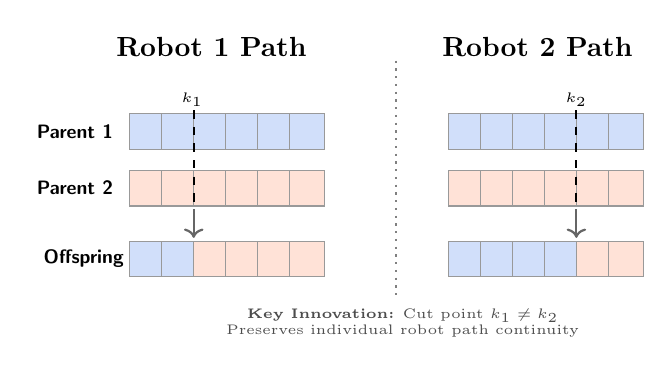
\begin{tikzpicture}[
    scale=0.9,
    font=\sffamily\scriptsize,
    % Box style for genome cells
    cell/.style={rectangle, draw=black!40, minimum width=0.45cm, minimum height=0.45cm, inner sep=0pt, outer sep=0pt},
    % Label style
    lbl/.style={anchor=east, font=\sffamily\bfseries\scriptsize}
]

    % --- ROBOT 1 COLUMN (Left) ---
    \node[font=\bfseries] at (0.9, 3.0) {Robot 1 Path};
    
    % Parent 1 (Blue)
    \node[lbl] at (-0.35, 1.8) {Parent 1};
    \foreach \i in {0,...,5} {
        \node[cell, fill=p1color!30] (r1p1_\i) at (\i*0.45, 1.8) {};
    }
    
    % Parent 2 (Orange)
    \node[lbl] at (-0.35, 1.0) {Parent 2};
    \foreach \i in {0,...,5} {
        \node[cell, fill=p2color!30] (r1p2_\i) at (\i*0.45, 1.0) {};
    }
    
    % Cut Line R1 (Index 2)
    \draw[dashed, thick, black] (0.65, 2.1) -- (0.65, 0.65);
    \node[font=\tiny] at (0.63, 2.25) {$k_1$};
    
    % Arrow
    \draw[->, thick, black!60] (0.65, 0.7) -- (0.65, 0.3);
    
    % Offspring R1 (Mix)
    \node[lbl] at (-0.2, 0) {Offspring};
    % First 2 from P1
    \foreach \i in {0,1} {
        \node[cell, fill=p1color!30] at (\i*0.45, 0) {};
    }
    % Rest from P2
    \foreach \i in {2,...,5} {
        \node[cell, fill=p2color!30] at (\i*0.45, 0) {};
    }


    % --- SEPARATOR ---
    \draw[dotted, thick, gray] (3.5, 2.8) -- (3.5, -0.5);


    % --- ROBOT 2 COLUMN (Right) ---
    \node[font=\bfseries] at (5.5, 3.0) {Robot 2 Path};
    
    % Parent 1 (Blue)
    \foreach \i in {0,...,5} {
        \node[cell, fill=p1color!30] (r2p1_\i) at (4.5 + \i*0.45, 1.8) {};
    }
    
    % Parent 2 (Orange)
    \foreach \i in {0,...,5} {
        \node[cell, fill=p2color!30] (r2p2_\i) at (4.5 + \i*0.45, 1.0) {};
    }
    
    % Cut Line R2 (Index 4 - Different form k1!)
    \draw[dashed, thick, black] (6.05, 2.1) -- (6.05, 0.65);
    \node[font=\tiny] at (6.05, 2.25) {$k_2$};
    
    % Arrow
    \draw[->, thick, black!60] (6.05, 0.7) -- (6.05, 0.3);
    
    % Offspring R2 (Mix)
    % First 4 from P1
    \foreach \i in {0,...,3} {
        \node[cell, fill=p1color!30] at (4.5 + \i*0.45, 0) {};
    }
    % Rest from P2
    \foreach \i in {4,5} {
        \node[cell, fill=p2color!30] at (4.5 + \i*0.45, 0) {};
    }

    % --- ANNOTATION ---
    \node[font=\tiny, align=center, text=black!70] at (3.6, -0.9) {
        \textbf{Key Innovation:} Cut point $k_1 \neq k_2$\\
        Preserves individual robot path continuity
    };

\end{tikzpicture}
\caption{Structure-Aware Crossover. Unlike standard crossover which cuts the entire genome once, we select independent cut points ($k_1, k_2$) for each robot, maintaining kinematic feasibility.}
\label{fig:crossover}
\end{figure}

\subsubsection{Ant Colony Optimization (ACO)}
We implemented an Ant System (AS) variant. The transition probability uses a pheromone trail $\tau_{ij}$ and a heuristic $\eta_{ij}$ favoring unexplored cells. The tuned baseline uses 30 ants for 200 iterations, evaporation $\rho=0.40$, pheromone weight $\alpha_{\tau}=0.5$, and heuristic weight $\beta_{\eta}=1.0$.

\subsubsection{Artificial Bee Colony (ABC)}
Adapted for discrete path planning with a colony size of 24 bees and 200 optimization cycles. Employed bees perturb paths using window-based mutation (window size 10, 5 retry attempts), and scouts reinitialize stagnating food sources (limit 12). Across our case studies, ABC is competitive with GA on some instances but achieves a lower average performance than ACO, motivating its inclusion as an optional portfolio member.

\FloatBarrier

\subsection{The Learned Router}
The Router is a Random Forest classifier trained on the collected router dataset ($N=9{,}179$). Labels are assigned to the algorithm achieving the minimum cost (ties broken by runtime). Class weighting is used to handle imbalance, and the SA decision threshold is tuned to $0.475$ to maximize SA one-vs-rest F1.

\section{Evaluation}
\label{sec:evaluation}

Experiments were conducted on $20 \times 20$ grid maps. The primary metrics were Coverage Percentage, Connectivity Score, and Disconnection Penalty. For router learning experiments, the current dataset uses fixed map statistics (empty map), focusing evaluation on connectivity and initial-team topology.

\subsection{Dataset and Experimental Protocol}
\label{sec:dataset_protocol}
For learning-based routing, we evaluate on the real router dataset collected by running SA, GA, ACO, and ABC on the same scenario and labeling each instance by the algorithm achieving the minimum objective cost (ties broken by runtime). We use the combined dataset with $N=9{,}179$ instances.

Each instance is generated by sampling the number of robots $R \in [2,6]$ and horizon $T \in [30,150]$, along with objective weights $(\alpha,\beta,\gamma)$ and connectivity parameters (communication radius and threshold). The optimization \emph{budget} for each solver is fixed to 50 iterations/generations (\texttt{budget}=50). In our current generator configuration, the map features are constant (\texttt{map\_height}=20, \texttt{map\_width}=20, \texttt{obstacle\_frac}=0, \texttt{unexplored\_frac}=1), so routing decisions are driven primarily by initial-team topology and constraint parameters.

We use a stratified $80/20$ train/test split with random seed 0, yielding $7{,}343$ training and $1{,}836$ test instances (Table~\ref{tab:router_dataset_split}). We report routing accuracy, the fail-safe critical error rate $\mathbb{P}(\hat{y}=\text{SA} \mid y=\text{ACO})$, and cost regret relative to the oracle-best solver for each instance.

\begin{table}[t]
    \centering
    \caption{Router dataset split and class counts ($N=9{,}179$).}
    \label{tab:router_dataset_split}
    \begin{tabular}{@{}lrrrrr@{}}
        \toprule
        \textbf{Split} & \textbf{Total} & \textbf{SA} & \textbf{GA} & \textbf{ACO} & \textbf{ABC} \\
        \midrule
        Train (80\%) & 7,343 & 862 & 2,481 & 3,978 & 22 \\
        Test (20\%)  & 1,836 & 216 & 620 & 991 & 9 \\
        \midrule
        All          & 9,179 & 1,078 & 3,101 & 4,969 & 31 \\
        \bottomrule
    \end{tabular}
\end{table}

\begin{table}[t]
\centering
\caption{Scenario parameter ranges in the router dataset (mean over $N=9{,}179$).}
\label{tab:router_param_ranges}
{
\setlength{\tabcolsep}{10pt} % applies only inside this group
\begin{tabular}{lccc}
\toprule
\textbf{Parameter} & \textbf{Min} & \textbf{Max} & \textbf{Mean} \\
\midrule
Robots $R$ & 2 & 6 & 3.88 \\
Horizon $T$ & 30 & 150 & 98.48 \\
$\alpha$ & 1.00e3 & 1.58e4 & 5.26e3 \\
$\beta$  & 1.00e2 & 1.58e3 & 5.38e2 \\
$\gamma$ & 0.50 & 10.00 & 5.28 \\
Comm. radius & 6.01 & 25.00 & 15.42 \\
Conn. threshold & 6.00 & 24.99 & 12.73 \\
\bottomrule
\end{tabular}
}
\end{table}


\subsection{Standalone Performance Comparison}
We benchmarked SA, GA, ACO, and ABC across 10 case studies with varying team sizes and horizons (Table~\ref{tab:case_study_summary}). ACO achieves the lowest cost in 9/10 scenarios and delivers the highest mean coverage. ABC wins one scenario (Case~9) and achieves competitive coverage on medium-sized problems, motivating its inclusion in the solver portfolio.

\begin{table}[t]
\centering
\caption{Aggregate performance across 10 case studies (lower cost is better).}
\label{tab:case_study_summary}
\begin{tabular}{@{}lccc@{}}
\toprule
\textbf{Algorithm} & \textbf{Mean Cost} & \textbf{Mean Coverage (\%)} & \textbf{Wins (Best Cost)} \\
\midrule
SA  & 32.1765 & 36.62 & 0/10 \\
GA  & 27.8834 & 43.75 & 0/10 \\
ACO & \textbf{21.0722} & \textbf{64.85} & \textbf{9/10} \\
ABC & 24.8959 & 46.85 & 1/10 \\
\bottomrule
\end{tabular}
\end{table}

\begin{figure}[t]
\centering
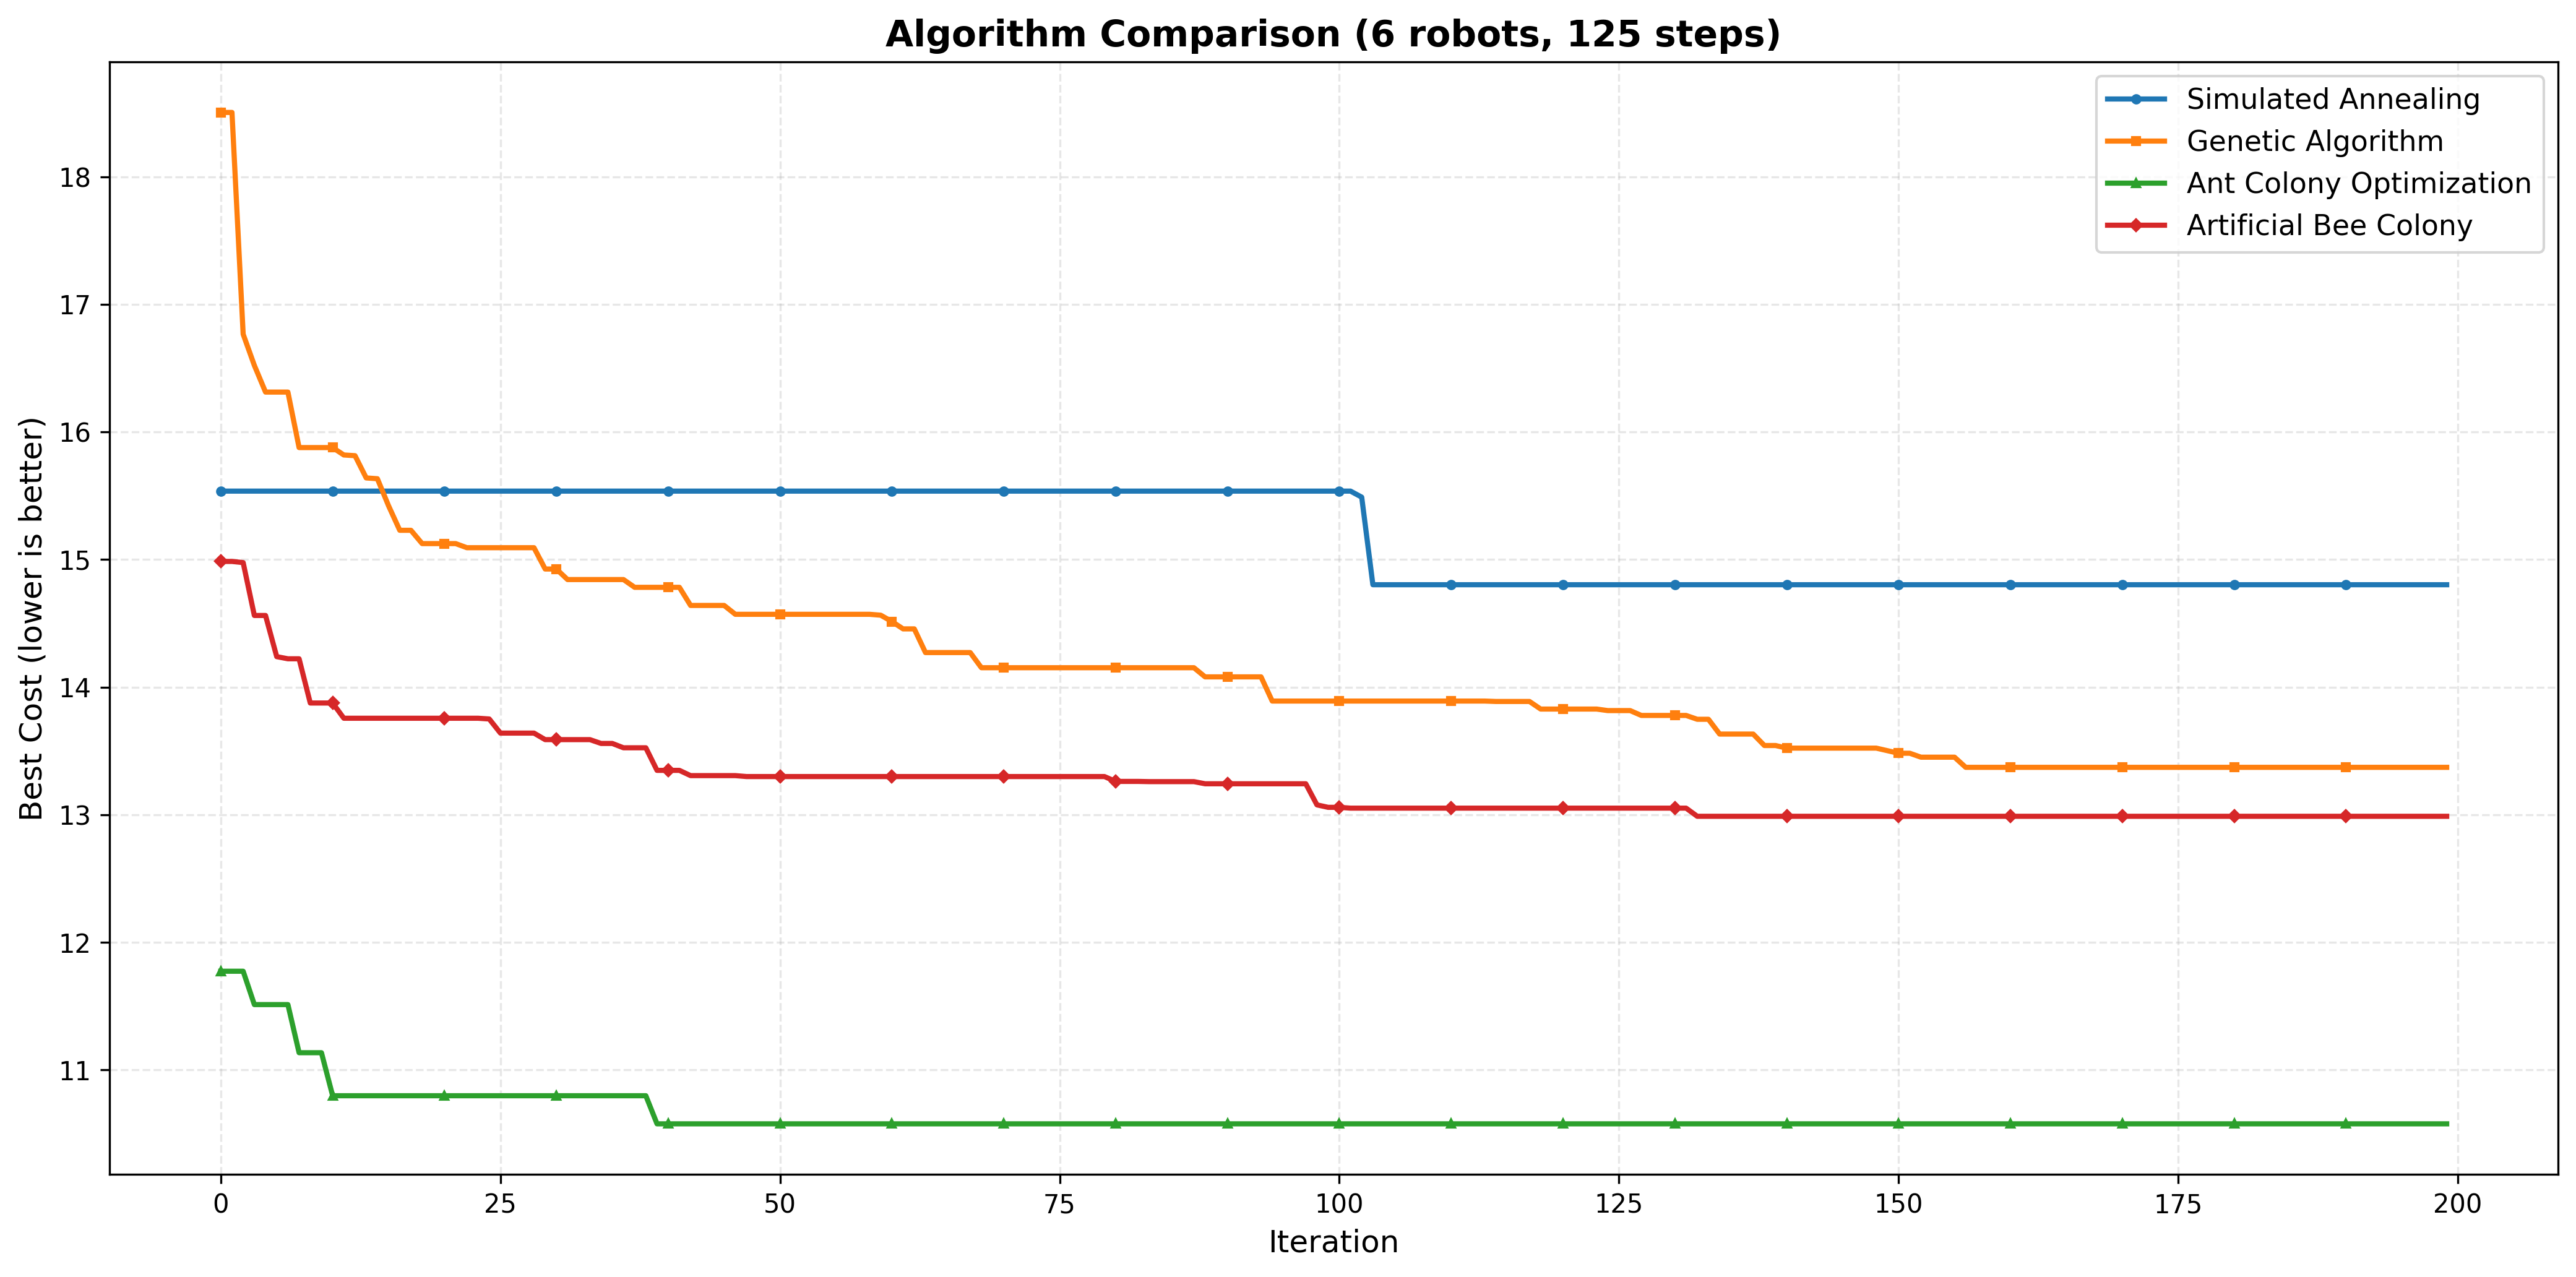
\includegraphics[width=0.48\textwidth]{Figures/case_study_1_comparison.png}
\caption{Convergence comparison for Case~1 (6 robots, 125 steps). ACO reaches the lowest final cost and highest coverage, while ABC is competitive with GA.}
\label{fig:case1_comparison}
\end{figure}

\subsubsection{Trajectory Visualization}
Aggregate metrics and convergence curves do not always convey \emph{how} robots distribute spatially. Fig.~\ref{fig:traj_visualization} shows qualitative examples of the resulting multi-robot trajectories and covered area on the grid, providing an intuitive view of constraint satisfaction (obstacle avoidance, no collisions) and team dispersion under connectivity pressure.

\begin{figure}[t]
\centering
\begin{minipage}[t]{0.48\columnwidth}
    \centering
    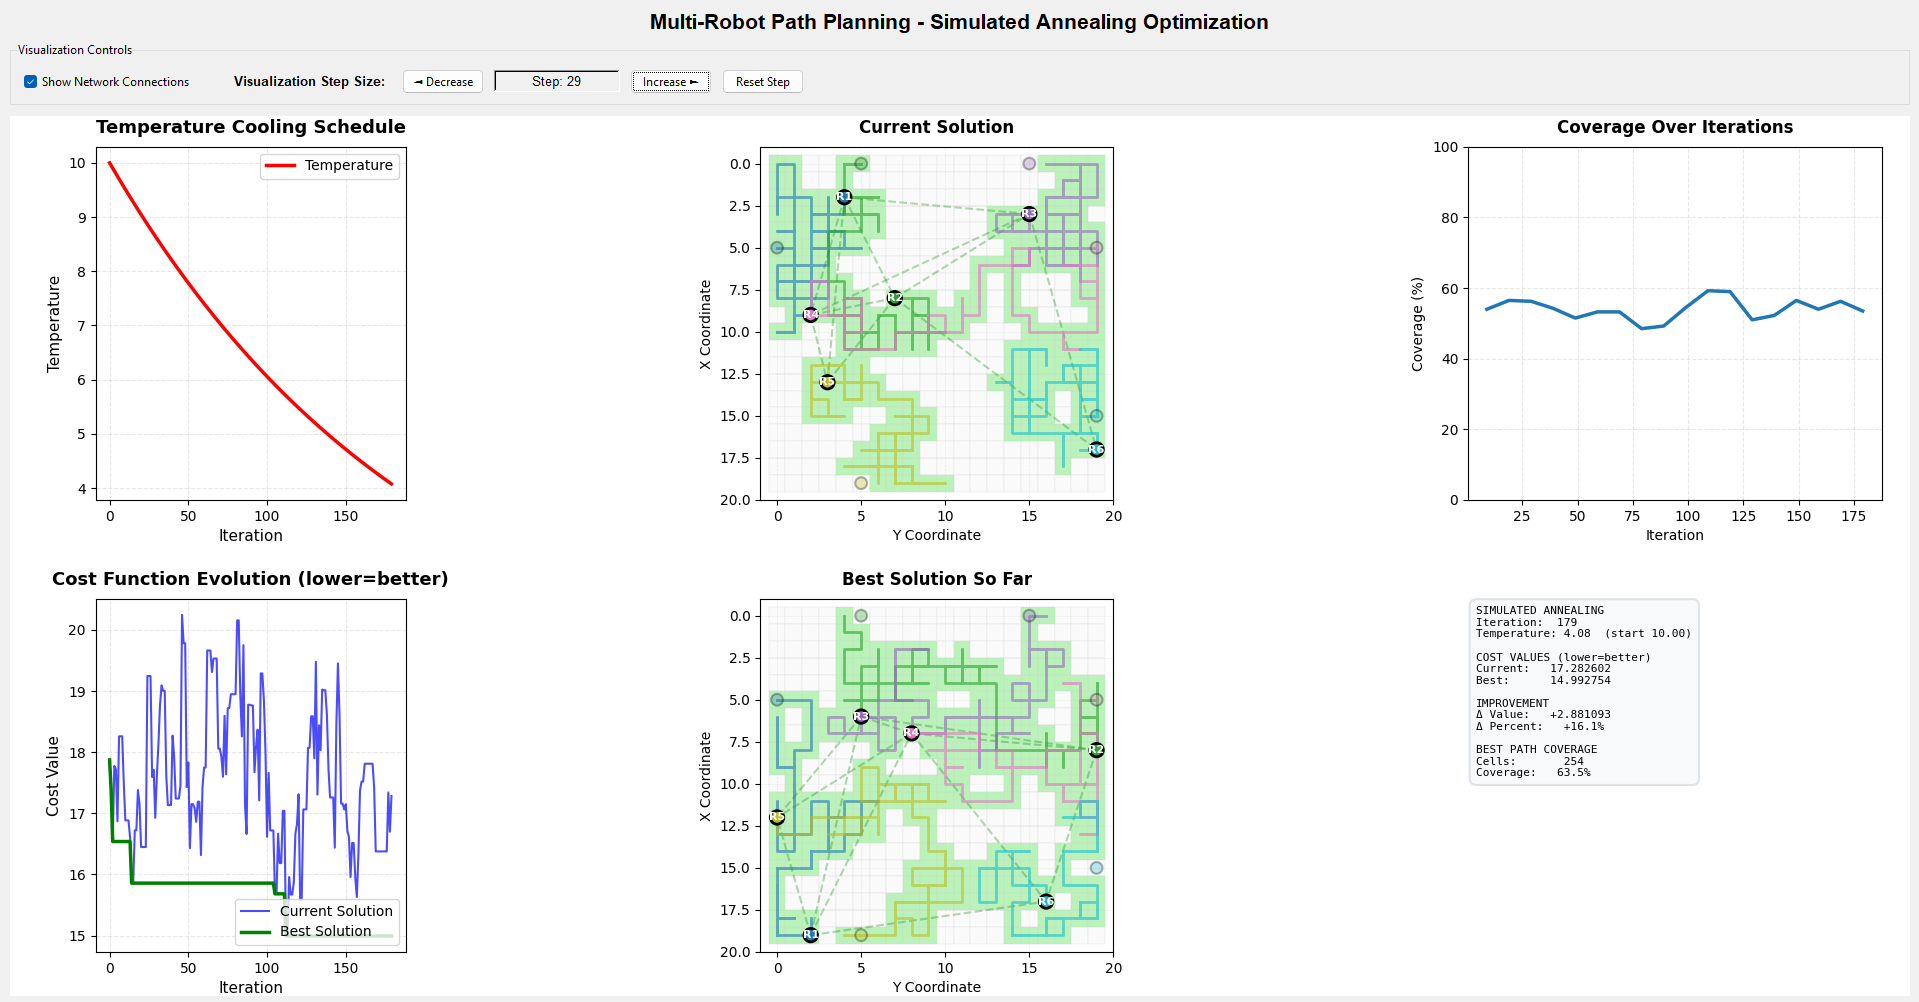
\includegraphics[width=\linewidth]{Figures/visualization.png}
\end{minipage}\hfill
\begin{minipage}[t]{0.48\columnwidth}
    \centering
    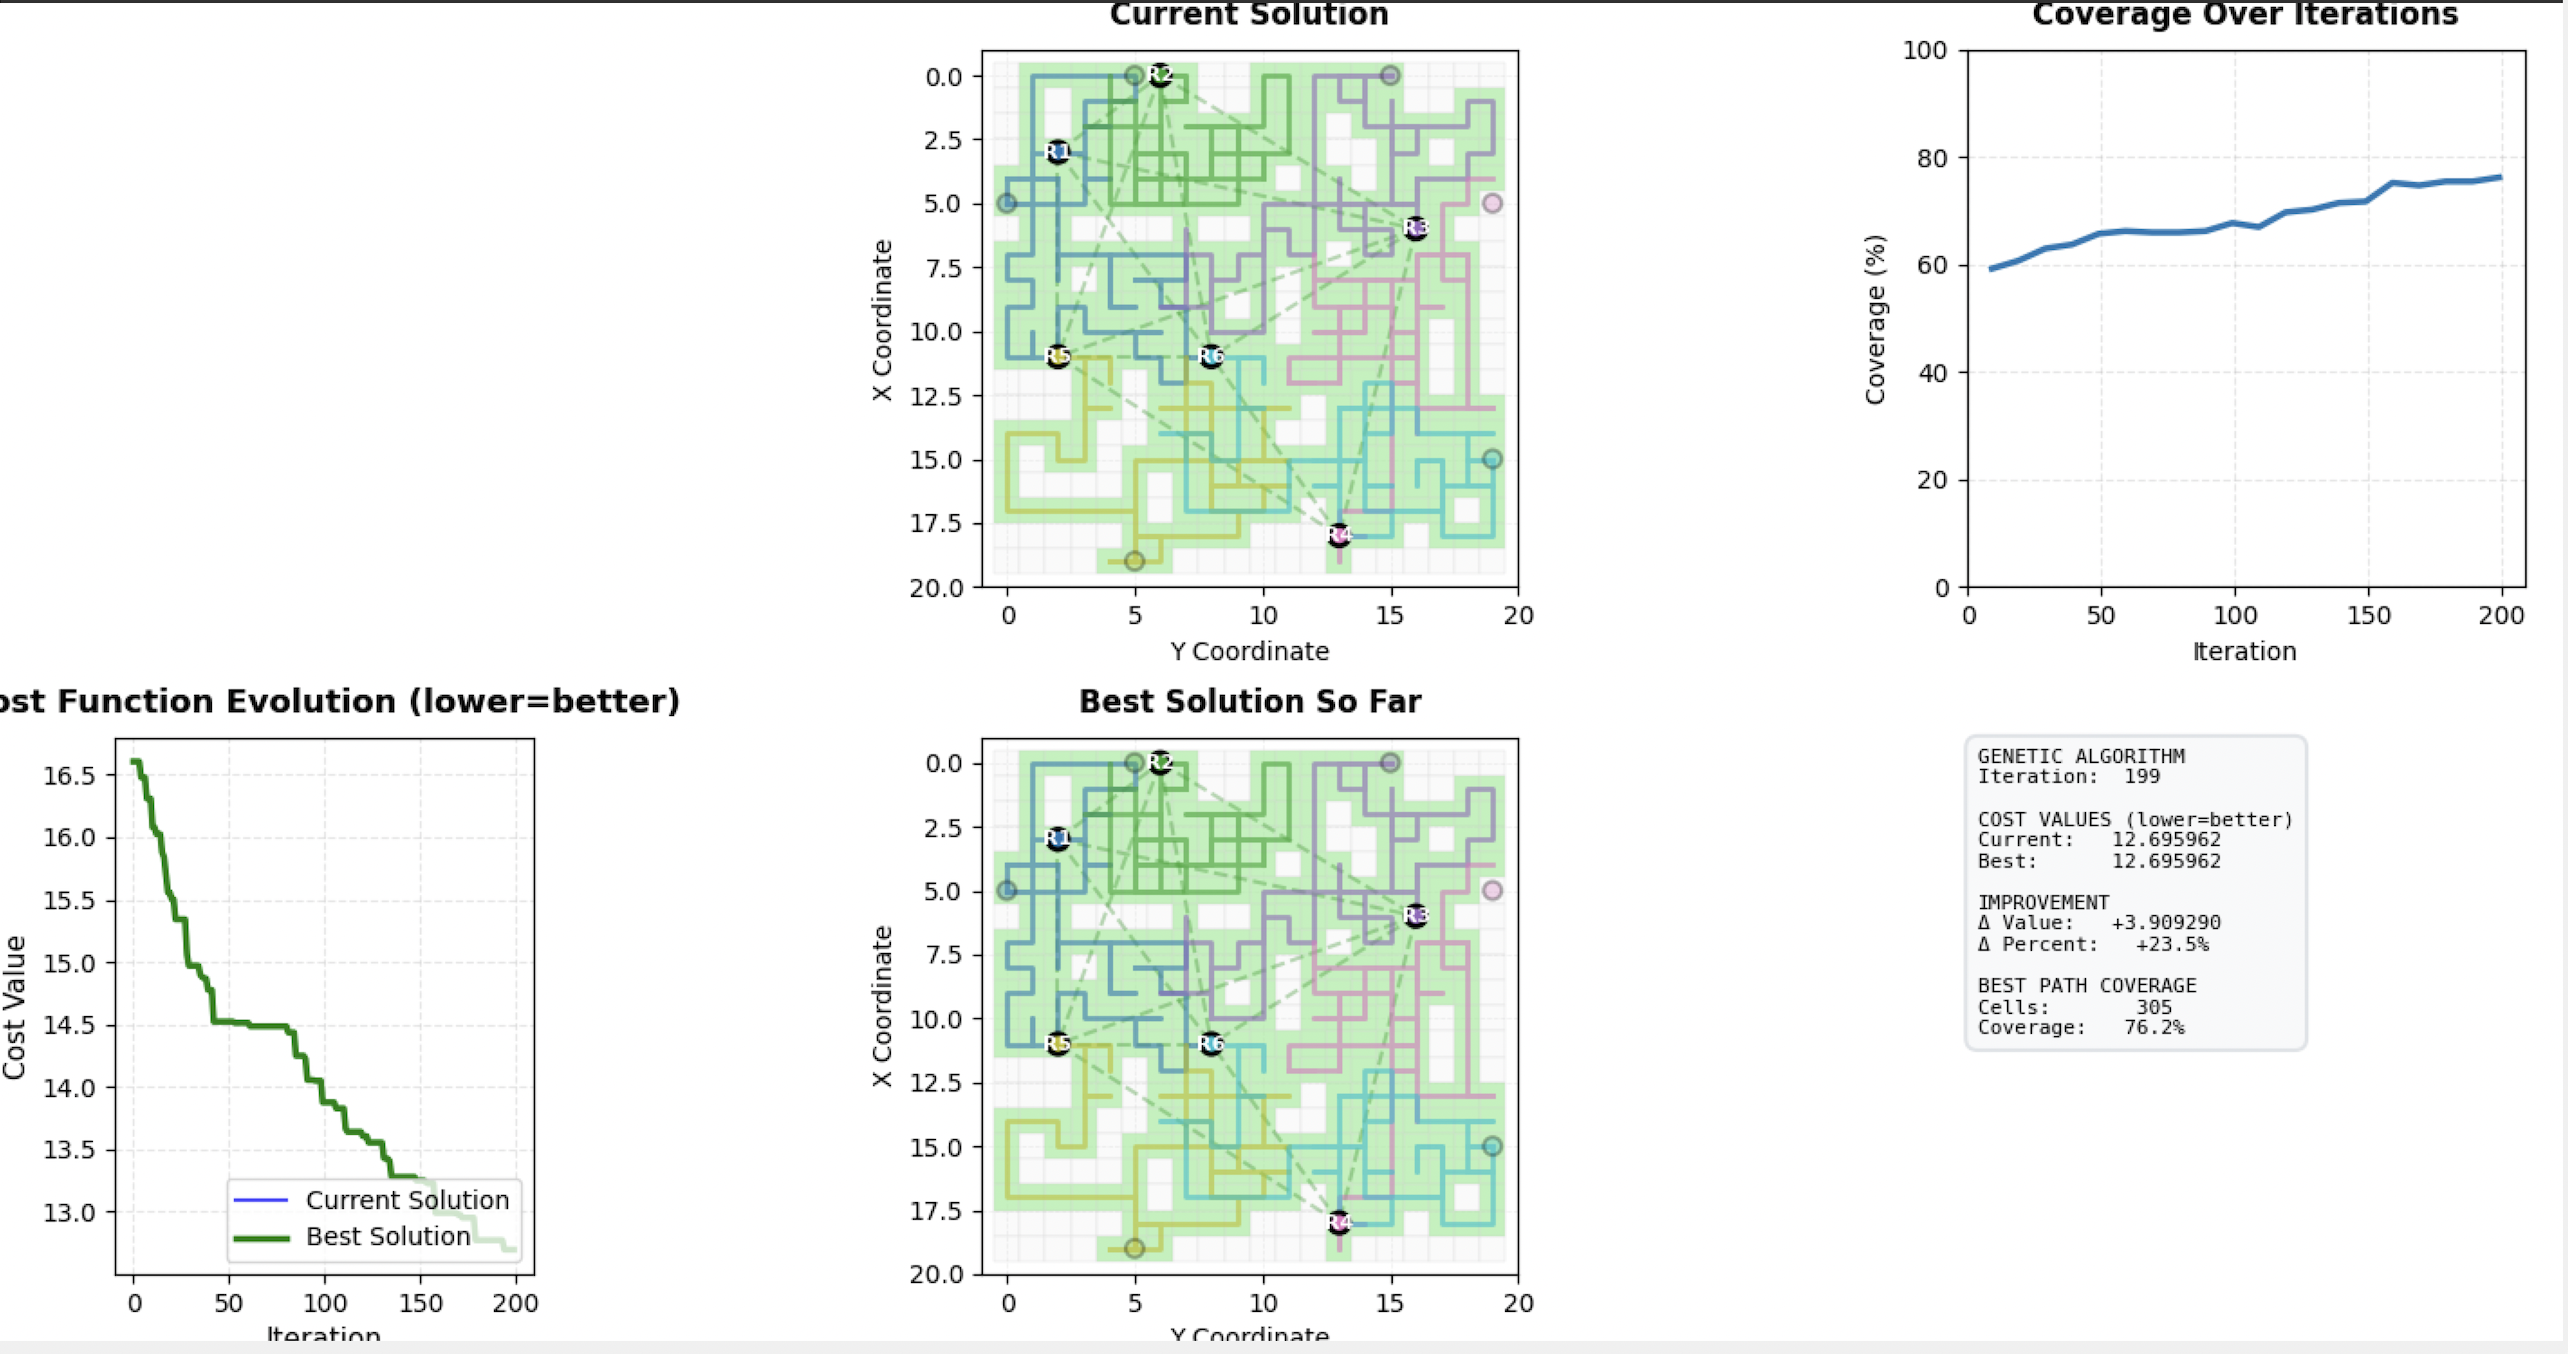
\includegraphics[width=\linewidth]{Figures/c1photo.png}
\end{minipage}
\caption{Example trajectory and coverage visualizations on the $20\times20$ grid. Left: SA solution illustrating fast but locally constrained exploration. Right: GA best-case (C1) showing coordinated dispersion while maintaining connectivity.}
\label{fig:traj_visualization}
\end{figure}

\subsubsection{Performance Indices}
To quantify solution quality, robustness, and computational efficiency, we report performance indices over 20 independent runs of each solver on the Case~1 configuration (6 robots, 125 steps, $\alpha=3000$, $\beta=500$, $\gamma=4.0$). Each run uses a different random seed/initial solution (SA/GA/ABC) or stochastic construction (ACO). Table~\ref{tab:performance_indices} summarizes the best cost, mean cost, standard deviation, and mean wall-clock time per run.

\begin{table}[t]
\centering
\caption{Performance indices over 20 independent runs on Case~1 (lower cost is better).}
\label{tab:performance_indices}
\small
\resizebox{\columnwidth}{!}{%
\begin{tabular}{@{}lcccc@{}}
\toprule
\textbf{Metric} & \textbf{SA} & \textbf{GA} & \textbf{ACO} & \textbf{ABC} \\
\midrule
Best cost & 13.7049 & 12.3180 & \textbf{11.4888} & 12.5941 \\
Mean cost & 14.3852 & 14.3379 & \textbf{11.7522} & 12.9810 \\
Std. dev. & $3.63{\times}10^{-1}$ & $2.19{\times}10^{0}$ & $1.13{\times}10^{-1}$ & $1.69{\times}10^{-1}$ \\
Mean time (s) & 34.867 & 165.515 & 130.991 & 69.035 \\
\bottomrule
\end{tabular}}
\end{table}

These indices reinforce the qualitative behavior seen in Fig.~\ref{fig:traj_visualization}: ACO delivers the best and most consistent solutions, SA is the fastest but lowest-quality solver, and ABC offers a favorable middle ground in runtime with competitive average cost.

\subsection{GA Hyperparameter Sensitivity}
To validate that GA performance is not an artifact of poor tuning, we varied the GA population size and number of generations under fixed weights ($\alpha=3000$, $\beta=500$) on the $20\times20$ grid (Table~\ref{tab:ga_sensitivity}). The best configuration in this sweep reaches 76.2\% coverage, but still trails tuned ACO (93.75\% coverage with the AS baseline).

\begin{table}[t]
\centering
\caption{GA sensitivity to population and generations (mutation rate = 30\%, elitism = 10\%).}
\label{tab:ga_sensitivity}
\begin{tabular}{@{}lcccc@{}}
\toprule
\textbf{Case} & \textbf{Pop.} & \textbf{Gens.} & \textbf{Coverage (\%)} & \textbf{Notes} \\
\midrule
C1 & 20 & 200 & \textbf{76.2} & Best \\
C2 & 10 & 200 & 65.5 & Low diversity \\
C3 & 30 & 200 & 71.0 & Diminishing returns \\
C4 & 20 & 100 & 68.5 & Under-converged \\
C5 & 20 & 300 & 70.8 & Longer run \\
C6 & 20 & 400 & 73.2 & Longer run \\
\bottomrule
\end{tabular}
\end{table}

\subsection{Router Training, Thresholding, and Calibration}
\label{sec:router_calibration}
The router is a Random Forest classifier trained on 17 instance features (Section~\ref{sec:features}) which contains a Random Forest with 200 trees, minimum leaf size 2, and \texttt{balanced\_subsample} class weighting. Since SA is a rare class, we apply a calibrated decision rule: we predict SA if its predicted probability exceeds a tuned threshold $t_{\text{SA}}$, otherwise we select the highest-probability non-SA solver. The threshold $t_{\text{SA}}$ is selected on a validation split to maximize SA one-vs-rest F1; the stored value is $t_{\text{SA}}=0.475$.

Calibration is important because the Router output is used as a \emph{decision} (especially for the rare SA class), not just as a label prediction: a poorly calibrated model can output overconfident SA probabilities on hard instances, increasing the risk of critical misrouting. To quantify confidence reliability, we report Expected Calibration Error (ECE) and multiclass Brier score on the held-out test set (Table~\ref{tab:router_calibration_metrics}). ECE measures the gap between predicted confidence and empirical accuracy across probability bins (lower is better), while the Brier score measures the mean squared error of predicted probability vectors (lower is better). The results indicate that predicted confidences are reasonably aligned with empirical accuracy (ECE $\approx 0.024$), while the SA one-vs-rest calibration is particularly tight (ECE $\approx 0.007$).

\begin{table}[t]
\centering
\caption{Router calibration metrics on the test set ($N=1{,}836$).}
\label{tab:router_calibration_metrics}
\begin{tabular}{p{0.65\linewidth} p{0.2\linewidth}}
\toprule
\textbf{Metric} & \textbf{Value} \\
\midrule
Top-1 ECE (10 bins) & 0.0244 \\
Multiclass Brier score & 0.0806 \\
SA one-vs-rest ECE (5 bins) & 0.0070 \\
\bottomrule
\end{tabular}
\end{table}


\subsection{Router Efficacy and Safety}
The Router demonstrated an accuracy of \textbf{94.99\%} on a held-out test set of 1,836 scenarios. 

\begin{figure}[t]
\centering
\def\cell{1.15}
\begin{tikzpicture}[
    scale=0.9,
    every node/.style={font=\sffamily\scriptsize},
    % Style for the heatmap boxes
    box/.style={draw=white, line width=0.9pt, rectangle, minimum size=\cell cm, align=center},
    % Style for axis labels
    axis_label/.style={font=\sffamily\bfseries\footnotesize},
    % Style for class labels
    class_label/.style={font=\sffamily\scriptsize}
]

    % --- DATA ---
    
    % Row 4: SA (Ground Truth)
    % Pred: SA(205), GA(8), ACO(1), ABC(2)
    \node[box, fill=primary!60] at (0, 3*\cell) {\textbf{205}\\[-1pt]\tiny (95\%)};
    \node[box, fill=primary!5]  at (1*\cell, 3*\cell) {\textbf{8}\\[-1pt]\tiny (4\%)};
    \node[box, fill=primary!2]  at (2*\cell, 3*\cell) {\textbf{1}\\[-1pt]\tiny (0\%)};
    \node[box, fill=primary!2]  at (3*\cell, 3*\cell) {\textbf{2}\\[-1pt]\tiny (1\%)};
    
    % Row 3: GA (Ground Truth)
    % Pred: SA(9), GA(570), ACO(39), ABC(2)
    \node[box, fill=primary!5]  at (0, 2*\cell) {\textbf{9}\\[-1pt]\tiny (1\%)};
    \node[box, fill=primary!55] at (1*\cell, 2*\cell) {\textbf{570}\\[-1pt]\tiny (92\%)};
    \node[box, fill=primary!10] at (2*\cell, 2*\cell) {\textbf{39}\\[-1pt]\tiny (6\%)};
    \node[box, fill=primary!2]  at (3*\cell, 2*\cell) {\textbf{2}\\[-1pt]\tiny (0\%)};
    
    % Row 2: ACO (Ground Truth) - FAIL SAFE ROW
    % Pred: SA(0), GA(35), ACO(965), ABC(0)
    \node[box, fill=green!10] (safe_cell) at (0, 1*\cell) {\textbf{0}\\[-1pt]\tiny (0\%)};
    \node[box, fill=primary!10] at (1*\cell, 1*\cell) {\textbf{35}\\[-1pt]\tiny (4\%)};
    \node[box, fill=primary!85, text=white] at (2*\cell, 1*\cell) {\textbf{965}\\[-1pt]\tiny (96\%)};
    \node[box, fill=green!10] (safe_cell_abc) at (3*\cell, 1*\cell) {\textbf{0}\\[-1pt]\tiny (0\%)};

    % Row 1: ABC (Ground Truth) - Rare Class
    % Pred: SA(0), GA(1), ACO(0), ABC(8)
    \node[box, fill=primary!2]   at (0, 0) {\textbf{0}\\[-1pt]\tiny (0\%)};
    \node[box, fill=primary!5]   at (1*\cell, 0) {\textbf{1}\\[-1pt]\tiny (11\%)};
    \node[box, fill=primary!2]   at (2*\cell, 0) {\textbf{0}\\[-1pt]\tiny (0\%)};
    \node[box, fill=abccolor!50] at (3*\cell, 0) {\textbf{8}\\[-1pt]\tiny (89\%)};

    % Highlight "fail-safe" cells with an inset outline (prevents overlap with neighboring cells)
    \draw[green!60!black, line width=0.6pt]
      ($(safe_cell.north west)+(0.05*\cell,-0.05*\cell)$) rectangle ($(safe_cell.south east)+(-0.15*\cell,0.15*\cell)$);
    \draw[green!60!black, line width=0.6pt]
      ($(safe_cell_abc.north west)+(0.05*\cell,-0.05*\cell)$) rectangle ($(safe_cell_abc.south east)+(-0.06*\cell,0.13*\cell)$);

    % --- LABELS ---
    
    % Column Labels (Predicted)
    \node[axis_label] at (1.5*\cell, 4.25*\cell) {Predicted Class};
    \node[class_label] at (0, 3.65*\cell) {SA};
    \node[class_label] at (1*\cell, 3.65*\cell) {GA};
    \node[class_label] at (2*\cell, 3.65*\cell) {ACO};
    \node[class_label] at (3*\cell, 3.65*\cell) {ABC};
    
    % Row Labels (Ground Truth)
    \node[axis_label, rotate=90] at (-1.85*\cell, 1.5*\cell) {Ground Truth};
    \node[class_label, anchor=east] at (-0.95*\cell, 3*\cell) {SA};
    \node[class_label, anchor=east] at (-0.95*\cell, 2*\cell) {GA};
    \node[class_label, anchor=east] at (-0.95*\cell, 1*\cell) {ACO};
    \node[class_label, anchor=east] at (-0.95*\cell, 0) {ABC};
    
    % Fail-Safe Annotation (left/below, routed to avoid overlaps)
    \node[font=\bfseries\tiny, text=green!40!black, align=center] (safe_txt) at (-2.05*\cell, -0.40*\cell) {Fail-Safe\\Verified};
    \coordinate (safe_mid) at (-0.75*\cell, -0.40*\cell);
    \draw[->, line width=0.7pt, green!40!black, shorten >=1pt] (safe_txt.east) -- (safe_mid) |- (safe_cell.mid west);

\end{tikzpicture}
\caption{Confusion Matrix on Test Set ($N=1836$). The diagonal shows high accuracy. Crucially, the bottom-left cell is \textbf{zero}, confirming that the router never assigns the lightweight solver (SA) to complex problems requiring ACO.}
\label{fig:confusion_matrix}
\end{figure}

The confusion matrix (Fig.~\ref{fig:confusion_matrix}) highlights the system's most critical property: \textbf{Fail-Safety}. 
In the 991 test cases where ACO was the ground-truth optimal solver (implying the problem was complex or obstacle-rich), the router \textbf{never} predicted SA ($0/991$ misclassifications). It only confused ACO with GA in 35 cases (3.5\%), which is an acceptable "soft failure" as GA is still a robust global solver. 

In contrast, predicting SA for an ACO-class problem would likely lead to mission failure (robots trapped in local minima). By virtually eliminating this specific error mode, \systemname{} proves suitable for autonomous deployment.

\begin{table}[t]
\centering
\caption{Comparison of Static vs. Adaptive Selection.}
\label{tab:router_performance}
\begin{tabular}{@{}lrrr@{}}
\toprule
Strategy & Win Rate (Oracle) & Precision & F1-Score \\
\midrule
Static (SA) & 11.7\% & 95.8\% & 96.0\% \\
Static (GA) & 33.8\% & 93.0\% & 93.0\% \\
Static (ACO) & \textbf{54.5\%} & 96.0\% & 96.0\% \\
Static (ABC) & 0.5\% & 94.0\% & 94\% \\
\textbf{\systemname{}} & \textbf{94.99\% (Acc)} & \textbf{95\% (Avg)} & \textbf{95\%} \\
\bottomrule
\end{tabular}
\end{table}


\subsection{Ablation Study}
\label{sec:ablations}
We evaluate several ablations to characterize which feature groups are essential for safe routing. Each ablation retrains the same Router model while removing a subset of the 17 features, then re-tunes the SA threshold $t_{\text{SA}}$ on a validation split for that feature set. Table~\ref{tab:router_ablations} reports accuracy, the fail-safe critical error rate (predicting SA when the oracle-best solver is ACO), mean relative regret, and the tuned SA threshold. We define the relative regret for an instance $S$ as:
\begin{equation}
    \text{RelRegret}(S) = \frac{J(\hat{y}(S)) - \min_{y \in \mathcal{Y}} J(y)}{\min_{y \in \mathcal{Y}} J(y) + \epsilon}
\end{equation}
where $J(\cdot)$ is the objective cost produced by a solver under the fixed budget, $\hat{y}(S)$ is the Router-selected solver, and $\mathcal{Y}$ is the solver portfolio.

Removing all topology features only slightly reduces accuracy, indicating that the constraint parameters alone already convey substantial instance difficulty. In contrast, restricting the router to topology and threshold features (7 features) significantly increases regret and introduces a small but non-zero critical error rate. Finally, a map-only router collapses to the class prior because map features are constant in this dataset, and it fails the fail-safe criterion.

\subsection{Feature Importance Analysis}
To understand the decision logic, we analyzed the Gini importance of the input features. 


The \textbf{Connectivity Threshold} (Importance $\approx 0.315$) and \textbf{Start Connectivity Edge Fraction} ($\approx 0.274$) are the dominant predictors, followed by minimum pairwise distances and horizon-related features. This aligns with our design intuition: when the initial communication graph is sparse (low edge fraction under the threshold), constructive search is required to recover connectivity, whereas dense initial graphs can be handled with lighter perturbative optimization.

\FloatBarrier

\section{Discussion}
\label{sec:discussion}

The results highlight a clear \emph{No Free Lunch} dynamic among the considered
optimizers: no single algorithm dominates across all multi-robot exploration
instances. Instead, performance depends strongly on instance characteristics,
particularly the density of the initial communication graph and the tightness of
connectivity constraints. \textbf{ACO} emerges as the primary workhorse, solving the
majority of challenging router instances ($\approx 54.5\%$) by effectively
reinforcing coordinated exploration through pheromone feedback. In contrast, \textbf{SA}
excels on simpler instances with dense connectivity ($\approx 11.8\%$), where its
fast convergence yields orders-of-magnitude runtime improvements. \textbf{GA} occupies a
robust middle ground, offering reliable performance across a broad range of
instances without specializing in extremes. \textbf{ABC} plays a niche but non-negligible
role, occasionally outperforming GA on medium-complexity instances with moderate
connectivity requirements, despite rarely being the globally optimal solver
($<1\%$).
These roles are further explained by the distinct optimization dynamics of each
method. \textbf{SA} converges rapidly but often plateaus early due to its single-solution
search. \textbf{GA} benefits from population-based recombination, enabling broad
exploration, yet remains sensitive to operator design and population diversity.
\textbf{ACO} consistently achieves superior coverage by combining heuristic initialization
with positive pheromone reinforcement, promoting coordinated multi-robot
behaviors. \textbf{ABC} occupies an intermediate regime: while its greedy local search
limits global optimality, its feasibility-preserving perturbations allow it to
remain competitive in later iterations when constraint satisfaction becomes the
dominant factor.
A limitation of this study is the fixed grid size ($20 \times 20$). However, the underlying combinatorial complexity ($4^{R \times T}$) remains extremely large, and the key topological features influencing router behavior—such as communication graph density and connectivity bottlenecks—are largely independent of scale. Consequently, we expect that the learned routing logic and the relative roles of the solvers will generalize effectively to larger environments.
\FloatBarrier

\begin{figure}[h] 
\centering
\makebox[\columnwidth][l]{%
\hspace{-2.8cm}%
\resizebox{1.35\columnwidth}{!}{%
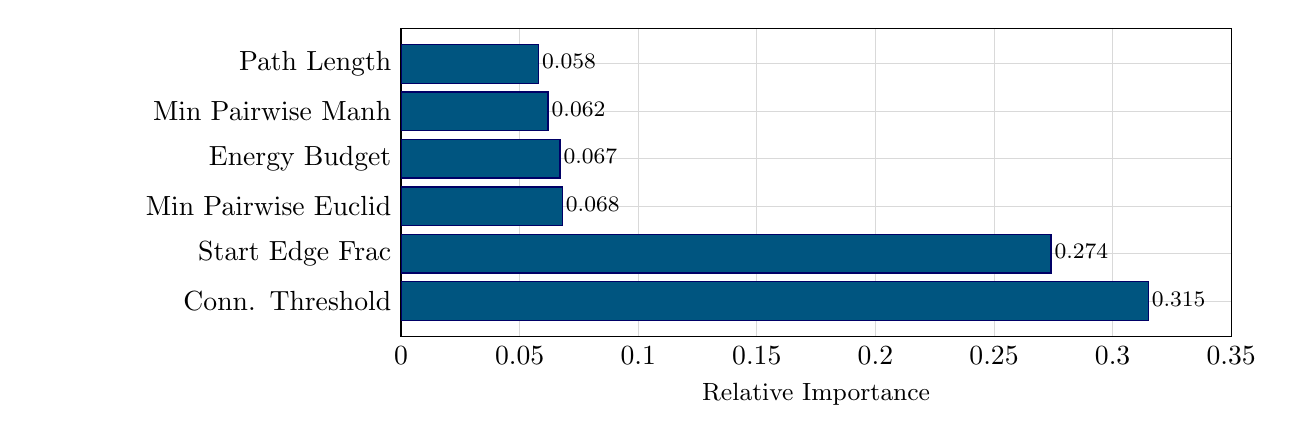
\begin{tikzpicture}
  \begin{axis}[
    xbar,
    width=\columnwidth,
    height=5.5cm,
    symbolic y coords={
      Conn. Threshold,
      Start Edge Frac,
      Min Pairwise Euclid,
      Energy Budget,
      Min Pairwise Manh,
      Path Length
    },
    ytick=data,
    xlabel={Relative Importance},
    xlabel style={font=\small},
    xmin=0, xmax=0.35,
    scaled x ticks=false,
    x tick label style={
      /pgf/number format/fixed,
      /pgf/number format/precision=2
    },
    nodes near coords,
    nodes near coords align={horizontal},
    nodes near coords style={
      font=\footnotesize,
      inner sep=-4pt,
      xshift=11pt
    },
    point meta=explicit symbolic,
    y tick label style={text width=4.5cm, align=right},
    bar width=14pt,
    grid=major,
    grid style={line width=0.3pt, gray!30},
    axis line style={-},
    tick style={major tick length=0pt},
    enlarge y limits=0.15
  ]
    \addplot[
      fill=primary,
      draw=blue!40!black,
      line width=0.5pt
    ] coordinates {
      (0.315,Conn. Threshold) [0.315]
      (0.274,Start Edge Frac) [0.274]
      (0.068,Min Pairwise Euclid) [0.068]
      (0.067,Energy Budget) [0.067]
      (0.062,Min Pairwise Manh) [0.062]
      (0.058,Path Length) [0.058]
    };
  \end{axis}
\end{tikzpicture}}}

\caption{Feature Importance (RF Gini). Connectivity threshold and start connectivity edge fraction dominate routing decisions. In this dataset, map features have zero importance because the map statistics are constant.}
\label{fig:feat_importance}
\end{figure}

\FloatBarrier

\section{Conclusion}
\label{sec:conclusion}

We presented \systemname{}, a connectivity-aware multi-robot path planning framework that leverages machine learning to adaptively select optimization strategies. Our evaluation confirms that the router achieves 94.99\% accuracy and exhibits a fail-safe capability, avoiding the selection of weak solvers for complex tasks. This reliability suggests that meta-learning routers are a viable path toward autonomous mission planning in heterogeneous environments.
Future work includes: (1) extending to dynamic obstacle environments, (2) incorporating real-time replanning triggers, (3) validating on physical robot platforms, and (4) exploring multi-objective routing beyond cost minimization.

\begin{table}[t]
\centering
\caption{Router ablations on the test set ($N=1836$).}
\label{tab:router_ablations}
\hspace{-0.7cm}%
\resizebox{1.1\columnwidth}{!}{%
\begin{tabular}{lcccc}
\toprule
\textbf{Variant} & \textbf{Acc.} &
\textbf{$\mathbb{P}(\hat{y}=\mathrm{SA}\mid y=\mathrm{ACO})$} &
\textbf{Mean Rel. Regret} & \textbf{$t_{\mathrm{SA}}$} \\
\midrule
Full (17 features) & 0.9499 & 0.0000 & 0.0639 & 0.475 \\
No topology (12) & 0.9483 & 0.0000 & 0.0634 & 0.595 \\
No weights (14) & 0.9466 & 0.0000 & 0.0376 & 0.440 \\
Topology + ($R$, threshold) (7) & 0.8851 & 0.0011 & 0.6615 & 0.455 \\
Map-only (4) & 0.1176 & 0.5447 & 5.0088 & 0.000 \\
\bottomrule
\end{tabular}}
\end{table}

% Prevent deferred figures/tables from appearing inside the references.
\FloatBarrier

\bibliographystyle{IEEEtran}
\begin{thebibliography}{00}

% Foundational Exploration
\bibitem{yamauchi1997frontier} B. Yamauchi, ``A frontier-based approach for autonomous exploration,'' in \textit{Proc. IEEE CIRA}, 1997.
\bibitem{stachniss2003iros} C. Stachniss and W. Burgard, ``Exploring unknown environments with mobile robots using coverage maps,'' in \textit{Proc. IJCAI}, 2003.

% Learning to Optimize / Selection
\bibitem{rice1976algorithm} J. R. Rice, ``The algorithm selection problem,'' \textit{Advances in Computers}, 1976.
\bibitem{hutter2014algorithm} F. Hutter et al., ``Algorithm runtime prediction: Methods \& evaluation,'' \textit{Artif. Intell.}, 2014.
\bibitem{chen2022learning} T. Chen et al., ``Learning to Optimize: A Primer and A Benchmark,'' \textit{J. Mach. Learn. Res.}, 2022.
\bibitem{zhu2023lero} R. Zhu et al., ``Lero: A Learning-to-Rank Query Optimizer,'' \textit{PVLDB}, 2023.

% Metaheuristics & Hybrid
\bibitem{deb2023multi} K. Deb and H. Jain, ``An evolutionary many-objective optimization algorithm using reference-point-based nondominated sorting approach, Part I: Solving problems with box constraints,'' \textit{IEEE Trans. Evol. Comput.}, 2014.
\bibitem{dorigo2024aco} M. Dorigo and T. St\"utzle, \textit{Ant Colony Optimization}. MIT Press, 2004.
\bibitem{kirkpatrick2021sa} S. Kirkpatrick, C. D. Gelatt, and M. P. Vecchi, ``Optimization by simulated annealing,'' \textit{Science}, 1983.
\bibitem{amet2025} ``Multi robot exploration using an advanced multi-objective salp swarm algorithm for efficient coverage and performance,'' \textit{Sci. Rep.}, 2025.

% Specifics
\bibitem{huang2020coverage} X. Huang et al., ``A Multi-Robot Coverage Path Planning Algorithm for the Environment With Multiple Land Cover Types,'' \textit{IEEE Access}, 2020.
\bibitem{kashyap2025simulations} G. S. Kashyap et al., ``From simulations to reality: enhancing multi-robot exploration for urban search and rescue,'' \textit{Int. J. Inf. Tech.}, 2025.
\bibitem{yan2023cooperative} Z. Yan et al., ``Multi-robot cooperative autonomous exploration via task allocation in terrestrial environments,'' \textit{Front. Neurorobot.}, 2023.
\bibitem{li2008swarm} Li et al., ``Robot swarm communication networks: architectures, protocols, and applications,'' in \textit{Proc. CHINACOM}, 2008.

\end{thebibliography}

\end{document}
